\chapter{Theoretical Background}%
\label{sec:theoretical_background}
% 2. Theoretical Background
% ==============================================================================

In order to understand the rest of the thesis, it is important to give a brief
overview of the fundamentals on which the kernels used are based on. This
section will cover the basics of neural networks and kernel methods.

\section{Extreme Learning Machines}%
\label{sub:neural_networks_fundamentals}
% 2.1 Extreme Learning Machines
% ==============================================================================
% Provide a brief overview of neural network architecture, including layers,
% nodes (neurons), activation functions, and the basic working principles.
% Explain how neural networks learn from data through processes like forward
% propagation and backpropagation.

Given $N$ distinct samples $\left( \textbf x_i,\, \textbf t_i \right)$,
where $\textbf x_i \in \mathbb{R}^n$ is the input vector and
$\textbf t_i \in \mathbb{R}^m$ is the target vector. Consider now a single layer
feedforward network (SLFN) with $\tilde{N}$ hidden nodes.
Let $\textbf w_i = \left[ w_{i1},\,w_{i2},\,\dots,\,w_{in} \right]^T$ be the
weight vector connecting the $i$-th hidden node to the input layer.
Let $\boldsymbol\beta_i = \left[ \beta_{i1},\,\beta_{i2},\,\dots,\,\beta_{im} \right]^T$
be the weight vector connecting the $i$-th hidden node to the output layer.
Finally, let $b_i$ be the bias of the $i$-th hidden node and $g(\cdot)$ be the
activation function.

We can model the model mathematically as follows:
\begin{equation}%
    \label{eq:slfn}
    \sum_{i=1}^{\tilde{N}} \boldsymbol\beta_{i} g\left( \textbf w_i \cdot \textbf x_j + b_i \right) = \textbf t_j, \quad j = 1,\,2,\,\dots,\,N
\end{equation}

\Cref{eq:slfn} can be rewritten in matrix form as:
\begin{equation}
    \textbf{H}\boldsymbol\beta = \textbf{T}
\end{equation}
where:
\begin{align}
    \textbf H        & = \begin{bmatrix}
                             g(\textbf w_1 \cdot \textbf x_1 + b_1) & g(\textbf w_2 \cdot \textbf x_1 + b_2) & \dots  & g(\textbf w_{\tilde{N}} \cdot \textbf x_1 + b_{\tilde{N}}) \\
                             g(\textbf w_1 \cdot \textbf x_2 + b_1) & g(\textbf w_2 \cdot \textbf x_2 + b_2) & \dots  & g(\textbf w_{\tilde{N}} \cdot \textbf x_2 + b_{\tilde{N}}) \\
                             \vdots                                 & \vdots                                 & \ddots & \vdots                                                     \\
                             g(\textbf w_1 \cdot \textbf x_N + b_1) & g(\textbf w_2 \cdot \textbf x_N + b_2) & \dots  & g(\textbf w_{\tilde{N}} \cdot \textbf x_N + b_{\tilde{N}})
                         \end{bmatrix}_{N \times \tilde{N}}, \\
    \boldsymbol\beta & = \begin{bmatrix}
                             \boldsymbol\beta_1 \\
                             \boldsymbol\beta_2 \\
                             \vdots             \\
                             \boldsymbol\beta_{\tilde{N}}
                         \end{bmatrix}_{\tilde{N} \times m}, \quad
    \textbf T = \begin{bmatrix}
                    \textbf t_1 \\
                    \textbf t_2 \\
                    \vdots      \\
                    \textbf t_N
                \end{bmatrix}_{N \times m}
\end{align}

The conventional way to train a SLFN is to use the backpropagation algorithm,
which is gradient based algorithm that aims to minimize the error $\left\lVert
    \textbf{T} - \textbf{H}\boldsymbol\beta \right\rVert$ by iteratively updating
the weights and biases of the network. This algorithm is computationally
expensive and can take a long time to converge.

\begin{figure}[htpb]
    % Single layer feedforward network
    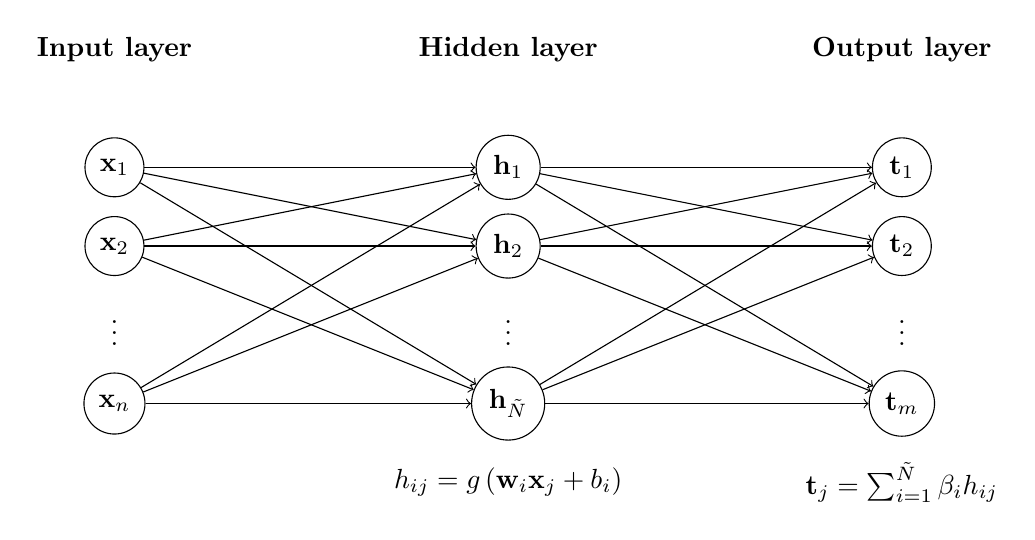
\begin{tikzpicture}
        % input layer
        \node[draw, circle] (x1) at (0, 0) {$\textbf x_1$};
        \node[draw, circle] (x2) at (0, -1) {$\textbf x_2$};
        \node (x3) at (0, -2) {$\vdots$};
        \node[draw, circle] (x4) at (0, -3) {$\textbf x_n$};

        % hidden layer
        \node[draw, circle] (h1) at (5, 0) {$\textbf h_1$};
        \node[draw, circle] (h2) at (5, -1) {$\textbf h_2$};
        \node (h3) at (5, -2) {$\vdots$};
        \node[draw, circle] (h4) at (5, -3) {$\textbf h_{\tilde{N}}$};

        % output layer
        \node[draw, circle] (y1) at (10, 0) {$\textbf t_1$};
        \node[draw, circle] (y2) at (10, -1) {$\textbf t_2$};
        \node (y3) at (10, -2) {$\vdots$};
        \node[draw, circle] (y4) at (10, -3) {$\textbf t_m$};

        \node (xtitle) at (0, 1.5) {\textbf{Input layer}};
        \node (htitle) at (5, 1.5) {\textbf{Hidden layer}};
        \node (ytitle) at (10, 1.5) {\textbf{Output layer}};

        \node (hformula) at (5, -4) {$h_{ij} = g \left( \textbf{w}_i \textbf{x}_j + b_i \right)$};
        \node (yformula) at (10, -4) {$\textbf{t}_{j} = \sum_{i=1}^{\tilde{N}} \boldsymbol\beta_{i} h_{ij}$};

        % connections
        \foreach \i in {1,2,4}
        \foreach \j in {1,2,4} {
                \draw[->] (x\i) -- (h\j);
                \draw[->] (h\i) -- (y\j);
            }
    \end{tikzpicture}
    \caption{Single layer feedforward network}%
\end{figure}

Extreme Learning Machines (ELMs) are an alternative training method for Single
Layer Feedforward Network (SLFN) in which the input weights $\textbf{w}_i$ and
hidden layer biases $b_i$ are randomly assigned. From that, the hidden layer
matrix $\textbf{H}$ can be computed, then the output weight $\boldsymbol\beta$
can be computed as $\boldsymbol\beta = \textbf{H}^{\dagger} \textbf{T}$, where
$\textbf{H}^{\dagger}$ is the Moore-Penrose pseudoinverse of $\textbf{H}$.
\Textcite{huangExtremeLearningMachine2006} showed that this method works for
activation functions that are infinitely differentiable.

ELM does is much faster to train than backpropagation, does not get stuck in
local minima and has better generalization performance. However the issue of
overfitting and underfitting is still present, and the performance of the
network is still dependent on the number of hidden nodes $\tilde{N}$.
\Textcite{huangExtremeLearningMachine2012} propose to incrementally add hidden
nodes and use cross-validation to determine the optimal number of hidden nodes.

\section{ELM Kernel (Arc-sine kernel)}%
\sectionmark{ELM Kernel}

\Textcite{frenayParameterinsensitiveKernelExtreme2011} expand on the idea of
ELMs \cite{huangExtremeLearningMachine2006,huangExtremeLearningMachine2012} by
changing the perspective and building a kernel from the ELM:
\begin{equation}
    k(x, z \mid p) = \frac{1}{p}\bigl\langle \phi(x),\,\phi(z) \bigr\rangle
\end{equation}
where $\phi(x)$ is the feature map of the ELM and $p$ is the number of hidden
nodes. Note that since ELM assigns the input weights $\textbf{w}_i$ and hidden
layer biases $b_i$ randomly, the feature space $\phi$ is also built randomly.
The authors show that in the limit of $p \to +\infty$, when the weights and
biases are drawn from a Gaussian distribution with variance $\sigma_w^2$, and
the activation function $g$ is the sigmoid \emph{erf} function defined in
\cref{eq:erf} and shown in \cref{fig:erf}, where it is compared to the
\emph{tanh} function, a very similar function also used in neural networks.
\begin{equation}\label{eq:erf}
    \erf(x) = \frac{2}{\sqrt{\pi}} \int_0^x e^{-t^2} \,dt
\end{equation}
Then, the asymptotic kernel $k$ can be analytically computed as shown in
\cref{eq:kernel_asin}:
\begin{equation}\label{eq:kernel_asin}
    k(\x,\,\z \mid p \to + \infty)  = \frac{2}{\pi}
    \arcsin \frac{1 + \left\langle \x,\,\z \right\rangle}{\sqrt{
            \left(
            \frac{1}{2\sigma_w^2} + 1 + \left\langle \x,\,\x \right\rangle
            \right)
            \left(
            \frac{1}{2\sigma_w^2} + 1 + \left\langle \z,\,\z \right\rangle
            \right)
        }}
\end{equation}

\begin{figure}[htpb]
    \begin{tikzpicture}
        \begin{axis}[
                every axis plot/.append style={smooth, mark=none, line width=1.5pt, domain=-3:3, samples=50, no markers},
                enlarge x limits=false,
                legend pos=north west,
                height=5cm,
                width=0.7\textwidth,
                grid=both,
                grid style={dotted, draw=gray!40, line width=1.0pt}
            ]
            \addplot+ gnuplot[id=erf]{erf(x)};
            \addlegendentry{$\erf(x)$};
            \addplot+[dashed] gnuplot[id=tanh]{tanh(x)};
            \addlegendentry{$\tanh(x)$};
        \end{axis}
    \end{tikzpicture}
    \caption{Comparison between the \emph{erf} and \emph{tanh} functions}
    \label{fig:erf}
\end{figure}

This kernel is the same as the one proposed by
\textcite{williamsComputationInfiniteNeural1998}\footnote{ In fact,
    \textcite{frenayParameterinsensitiveKernelExtreme2011} reference
    \textcite{williamsComputationInfiniteNeural1998} as the source of the
    analytical expression.
}, which is derived from a different perspective. In this older paper by
\citeauthor{williamsComputationInfiniteNeural1998}, the kernel formulation comes
from applying the principles of Bayesian Learning to neural
networks\cite{nealBayesianLearningNeural1996,bishopBayesianNeuralNetworks1997}.

Bayesian Neural Networks (BNN) are neural networks that make use of the Bayesian
Machinery to learn from data. The main difference is that these networks use
distributions instead of point estimates\cite{nealBayesianLearningNeural1996}.
This allows the network to have a better understanding of the uncertainty of the
data, which reduces overfitting and allows having uncertainty estimates for the
predictions. The main drawback of BNNs is that they require computation of the
posterior distribution, which is an analytically intractable integral.
Therefore, they are trained using approximate methods such as Markov Chain Monte
Carlo (MCMC) which are computationally expensive and slow to converge
\cite{nealBayesianTrainingBackpropagation1992}.
\Textcite{williamsComputationInfiniteNeural1998} shows that in the limit of
infinitely wide neural networks, when the weights and biases are drawn from a
Gaussian distribution, and the activation function is the sigmoid \emph{erf}, an
analytical expression for the covariance matrix can be derived.

\subsection{Analytical expression for the ELM kernel}

In this section I summarize the main results from
\textcite{williamsComputationInfiniteNeural1998} for the analytical expression
of a single layer bayesian network with a sigmoid \emph{erf} activation function
and Gaussian priors on the weights and biases. Such construction is equivalent
to the ELM kernel proposed by
\textcite{frenayParameterinsensitiveKernelExtreme2011}.

The basis of the derivation follows from the results of
\textcite{mackayBayesianMethodsAdaptive1999,nealBayesianTrainingBackpropagation1992}
which using Bayesian machinery. From there and using \emph{erf} (\cref{eq:erf})
as the activation function and assuming that the input to hidden weights
$\textbf u$ are drawn from a zero-mean Gaussian distribution with covariance
matrix $\boldsymbol\Sigma$, \citeauthor{williamsComputationInfiniteNeural1998}
obtains the following expression for the covariance matrix:
\begin{equation}\label{eq:integral_williams}
    V_{\erf}\left(\x,\,\x'\right) = \frac{1}{(2\pi)^{\frac{d+1}{2}}|\boldsymbol\Sigma|^{\frac{1}{2}}}
    \int
    \erf \left(\textbf u^T \tilde \x\right)
    \erf \left(\textbf u^T \tilde \x'\right) \times \exp \left(
    -\frac{1}{2} \textbf u^T \boldsymbol\Sigma^{-1} \textbf u
    \right) \,d\textbf u
\end{equation}
then, in the appendix, \citeauthor{williamsComputationInfiniteNeural1998} shows
that the integral can evaluated to the expression shown in
\cref{eq:kernel_asin}.

% TODO: Maybe some more details on how he gets to the expression

\section{Arc-cosine kernels}

\Textcite{choLargemarginClassificationInfinite2010} generalize the work of
\textcite{williamsComputationInfiniteNeural1998} by expanding the family of
infinite neural network kernels to include other activation functions. Their
formulation starts from the following integral:
\begin{equation}\label{eq:integral_cho}
    k_n(\x, \y) = 2 \bigintss \frac{\exp\left(-\frac{\lVert \textbf w \rVert^2}{2}\right)}{(2\pi)^{d/2}}
    \Theta(\textbf w \cdot \x) \Theta(\textbf w \cdot \y) (\textbf w \cdot \x)^n (\textbf w \cdot \y)^n \,d\textbf w
\end{equation}
where $\Theta(z) = \frac{1}{2} \bigl(1 + \text{sign}(z)\bigr)$ is the Heaviside
step function. And $n$ is a hyperparameter corresponding to the order of the
kernel. In this kernel, $\Theta(z)z^n$ is the activation function of the neural
network, which varies depending on the value of $n$ as shown in
\cref{fig:activation_functions}.

Notice the similarities between this integral (\cref{eq:integral_cho}) and the
previous one from \citeauthor{williamsComputationInfiniteNeural1998}
(\cref{eq:integral_williams}). The main difference between the two is the
activation function and the fact that
\citeauthor{williamsComputationInfiniteNeural1998} uses a general covariance
matrix $\boldsymbol\Sigma$ while
\citeauthor{choLargemarginClassificationInfinite2010} uses a diagonal covariance
matrix $\boldsymbol\Sigma = \sigma_w^2 \textbf I$.
\Citeauthor{choLargemarginClassificationInfinite2010} show that their
formulation when $n=0$ can be derived from a specialization of the formulation
from \textcite{williamsComputationInfiniteNeural1998}.

The integral in \cref{eq:integral_cho} can be only computed for $n >
    -\frac{1}{2}$. However, for $n < 0$, the behaviour is unintuitive, as the kernel
map the origin in the input space to infinity in the feature space (and there is
no analytical expression for the kernel).

\begin{figure}[H]
    \begin{tikzpicture}
        \begin{groupplot}[group style={
                        group size=3 by 1,
                        xlabels at=edge bottom,
                        ylabels at=edge left,
                        vertical sep=4em,
                    },
                width = .3\textwidth,
                ymin=-0.1, ymax=1.1,
                every axis plot/.append style={smooth, mark=none, line width=2pt},
                enlarge x limits=false,
                samples=25,
                domain=-1:1,
                xmin=-1, xmax=1,
                grid=both,
                grid style={dotted, draw=gray!40, line width=1.0pt}
            ]
            \nextgroupplot[title={\bfseries Step $(n = 0)$}]
            \draw[line width=2pt, color=blue] (-1,0) -- (0,0);
            \draw[line width=2pt, color=blue, dashed] (0,0) -- (0,1);
            \draw[line width=2pt, color=blue] (0,1) -- (1,1);

            \nextgroupplot[title={\bfseries Ramp $(n=1)$}]
            \draw[line width=2pt, color=red] (-1,0) -- (0,0) -- (1.1,1.1);

            \nextgroupplot[title={\bfseries Quarter-pipe $(n=2)$}]
            \draw[line width=2pt, color=green!70!black] (-1,0) -- (0,0);
            \addplot[domain=0:1.1, line width=2pt, color=green!70!black] {x^2};
        \end{groupplot}
    \end{tikzpicture}
    \caption{Activation functions $\Theta(z)z^n$ for $n = 0,\,1,\,2$}
    \label{fig:activation_functions}
\end{figure}

More interestingly, they show that an analytical expression for the
kernel can be derived for $n \in \left\{ 0,\,1,\,2,\,\dots \right\}$
and provide such expressions for $n = 0,\,1,\,2$. This expression has a simple
relationship with the magnitude of the input vectors $\x$ and $\y$ and a more
complex one with the angle between them:
\begin{equation}\label{eq:kernel_cho}
    k_n(\x,\,\y) = \frac{1}{\pi} \left\lVert \x \right\rVert^n \left\lVert \y \right\rVert^n J_n(\theta)
\end{equation}
where $\theta$ is the angle between $\x$ and $\y$ and $J_n(\theta)$ is the more complex
part of the expression:
\begin{equation}
    J_n(\theta) = (-1)^n \left( \sin \theta \right)^{(2n+1)}
    \left( \frac{1}{\sin \theta} \frac{\partial}{\partial \theta} \right)^2
    \left( \frac{\pi - \theta}{\sin \theta} \right)
    \quad \text{for} \quad \forall n \in \left\{ 0,\,1,\,2,\,\dots \right\}
\end{equation}
For $n = 0,\,1,\,2$, the expression for $J_n(\theta)$ is:
\begin{align}
    J_0(\theta) & = \pi - \theta                                                                    \\
    J_1(\theta) & = \sin\theta + \left(\pi - \theta\right)\cos\theta                                \\
    J_2(\theta) & = 3\sin\theta\cos\theta + \left(\pi - \theta\right)\left(1 + 2\cos^2\theta\right)
\end{align}

From these, and using $\theta = \arccos\frac{\x \cdot \y}{\left\lVert \x
        \right\rVert \left\lVert \y \right\rVert}$ we get the expression for the first
three kernels:
\begin{align}
    \label{eq:kernel_cho_n0}
    k_0(\x,\,\y) & = 1 - \frac{1}{\pi} \arccos\frac{\x \cdot \y}{\left\lVert \x \right\rVert \left\lVert \y \right\rVert} \\
    \label{eq:kernel_cho_n1}
    k_1(\x,\,\y) & = \frac{1}{\pi} \left\lVert \x \right\rVert \left\lVert \y \right\rVert
    \bigl( \sin\theta + \left(\pi - \theta\right)\cos\theta \bigr)                                                        \\
    \label{eq:kernel_cho_n2}
    k_2(\x,\,\y) & = \frac{1}{\pi} \left\lVert \x \right\rVert^2 \left\lVert \y \right\rVert^2
    \Bigl( 3\sin\theta\cos\theta + \left(\pi - \theta\right)\left(1 + 2\cos^2\theta\right) \Bigr)
\end{align}

\subsection{Covariance arc cosine kernel}

The formulation from \textcite{choLargemarginClassificationInfinite2010} is
derived from a standard normal distribution (i.e. mean 0 and variance 1).
\Textcite{pandeyGoDeepWide2014} show that if instead the samples are drawn from
a gaussian distribution with mean 0 and covariance $\Sigma$, then the kernel
$K_{\Sigma,\,n}$ is related to the original kernel $K_{n}$ as follows:
\begin{equation}\label{eq:kernel_pandey}
    K_{\Sigma,\,n}(\x,\,\y) = K_{n}\left(\Sigma^{\frac{1}{2}}\x,\,\Sigma^{\frac{1}{2}}\y\right)
\end{equation}

\section{Kernel normalization}%
% TODO: why is this usefull? the original kernel seems to work fine in practice
% and a priori seems already normalized?

\Textcite{frenayParameterinsensitiveKernelExtreme2011} do not use the expression
of the arc-sine kernel from \cref{eq:kernel_asin} directly. Instead, they use
the normalized version. The normalization of a kernel is defined as follows:
\begin{equation}\label{eq:kernel_normalization}
    K'(\x,\,\y) = \frac{K(\x,\,\y)}{\sqrt{K(\x,\,\x)K(\y,\,\y)}}
\end{equation}

